\section{Experiments}

%We will first introduce the experiment setting, then show the results and analysis on the two types of datasets respectively.

\subsection{Experiment Setting}

%\subsubsection{Dataset.} We conduct our experiments on two real-world datasets, whose statistics are summarized in Table 2. These databases have different characteristics and evolution behaviour. We also consider different type of target relationship as discussed in subsection \ref{targetRelashipSection}.
\subsubsection{Dataset.} We conduct our experiments on two real-world datasets that have different characteristics and evolution behaviour. 


\begin{itemize}
    \item \textit{Publications dataset:} The \textit{aminer} citation dataset\footnote{\url{https://aminer.org/citation}} V8 (2016-07-14) is extracted from DBLP, ACM, and other sources. It contains 3,272,991 papers and 8,466,859 citation relationships for 1,752,443 authors, who published in 10,436 venues, from 1930 to 2016. Each paper is associated with abstract, authors, year, venue, and title. \amin{We consider only those papers published since 1996, which includes X papers and Y authors.} Authors in \cite{sun2011ASONAM} used a similar dataset but considered only authors with more than 5 publications. We generate two datasets: one that contains all publications, and one that considers authors with at least 5 papers. We consider $k=3, 5, and 10$ different time intervals for the dynamic analysis. In our evaluation, we execute the learned model on the last interval to measure the prediction accuracy.
    
    \item \textit{Movies dataset:} The RecSys HetRec 2011 movie data set \cite{Cantador:RecSys2011} is an extension of MovieLens10M dataset, published by GroupLeans research group \footnote{\url{http://www.grouplens.org}} that links the movies of MovieLens dataset with their corresponding web pages at Internet Movie Database (IMDb\footnote{\url{http://www.imdb.com}}) and Rotten Tomatoes\footnote{\url{http://www.rottentomatoes.com}} movie review systems. It contains information of 2,113 users, 10,197 movies, 20 movie genres (avg. 2.04 genres per movie), 4,060 directors, 95,321 actors (avg. 22.78 actors per movie), 72 countries, 855,598 ratings (avg. 404.92 ratings per user, and avg. 84.64 ratings per movie), and 13,222 tags (avg. 22.69 tas per user, avg. 8.12 tas per movie).

\end{itemize}


%\textbf{Publications dataset:} The \textit{aminer} citation dataset\footnote{\url{https://aminer.org/citation}} V8 (2016-07-14) is extracted from DBLP, ACM, and other sources. It contains 3,272,991 papers and 8,466,859 citation relationships for 1,752,443 authors, who published in 10,436 venues, from 1930 to 2016. Each paper is associated with abstract, authors, year, venue, and title. \amin{We consider only those papers published since 1996, which includes X papers and Y authors.} Authors in \cite{sun2011ASONAM} used a similar dataset but considered only authors with more than 5 publications. We generate two datasets: one that contains all publications, and one that considers authors with at least 5 papers. We consider $k=3, 5, and 10$ different time intervals for the dynamic analysis. In our evaluation, we execute the learned model on the last interval to measure the prediction accuracy.

%The ml-latest-small\footnote{\url{http://files.grouplens.org/datasets/movielens/ml-latest-small-README.html}} dataset describes 5-star rating and free-text tagging activity from MovieLens\footnote{\url{https://movielens.org/}}, a movie recommendation service. It contains 100004 ratings and 1296 tag applications across 9125 movies. These data were created by 671 users between January 09, 1995 and October 16, 2016. This dataset was generated on October 17, 2016.

%\textbf{Movies dataset:} The RecSys HetRec 2011 movie data set \cite{Cantador:RecSys2011} is an extension of MovieLens10M dataset, published by GroupLeans research group \footnote{\url{http://www.grouplens.org}} that links the movies of MovieLens dataset with their corresponding web pages at Internet Movie Database (IMDb\footnote{\url{http://www.imdb.com}}) and Rotten Tomatoes\footnote{\url{http://www.rottentomatoes.com}} movie review systems. It contains information of 2,113 users, 10,197 movies, 20 movie genres (avg. 2.04 genres per movie), 4,060 directors, 95,321 actors (avg. 22.78 actors per movie), 72 countries, 855,598 ratings (avg. 404.92 ratings per user, and avg. 84.64 ratings per movie), and 13,222 tags (avg. 22.69 tas per user, avg. 8.12 tas per movie).


Movies once release, users can rate them but a paper is published once and new co-authorship is made only at that time.

In co-authorship all connections are new in MovieDB new connections to an existing movie. This is a common problem with all rating datasets.

%Datasets of different sizes.
We also conduct our experiments on two variations of the DBLP, one with min 5paper as in ... and one with all.


\subsubsection{Taget relationships.} We consider different type of target relationship.

Network schema for the two datasets are shown in Figure X. Note that we consider a simplified version and ignore nodes such as topic fro papers or tag for movies.


\begin{figure}[t]
\centering
\subfigure[DBLP]{
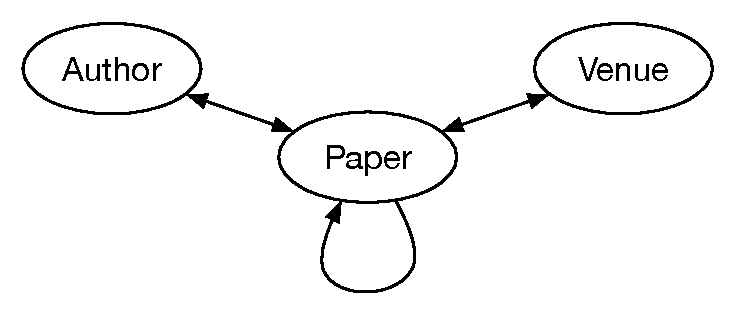
\includegraphics[trim = 0mm 0mm 0mm 0mm,width=0.47\hsize]{figs/publicationsSchema.pdf}
 \label{Fig:DBLP}
}
\subfigure[IMDB]{
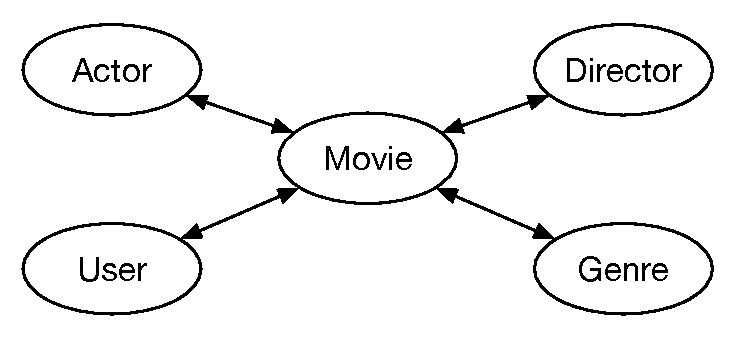
\includegraphics[trim = 0mm 0mm 0mm 0mm,width=0.47\hsize]{figs/moviesSchema.pdf}
 \label{Fig:IMDB}
}
\caption{The simplified network schema used for our experiments.} \label{Fig:expSchema}
\end{figure}


We consider .... based on the work in ... we con

Authors in \cite{sun2011ASONAM} conducted Wald test in a case study and found that the p-value for the feature associated with each meta path and their significance level. From the results, we can see that the shared co-authors, shared venues, shared topics and co-cited papers for two authors all play very significant roles in determining their future collaboration(s). For...

Similarly we only calculated the PC for these meta paths. Note that the goal of our paper is not to select the best features but to show the strength of using...

Table \ref{table_publications} shows meta paths between authors under length 4 for the publications dataset.


\begin{table}[h]
\centering
\caption{Publications Dataset Meta Paths (\textit{A} = author, \textit{P} = paper, \textit{A} = venue).}
\label{table_publications}
\begin{tabular}{|c|l|} \hline
\textbf{Meta path} & \textbf{Meaning} \\ \hline

\textit{A--P--A} & [\textit{The target relation}] Authors are coauthors \\ \hline
\textit{A--P--V--P--A} & Authors publish in the same venue \\ \hline
\textit{A--P--A--P--A} & Authors have the same co-author \\ \hline
\textit{A--P--P--P--A} & Authors cite the same papers \\ \hline

\end{tabular}
\end{table}

Unlike the \textit{A--P--A} target relation for the publication dataset for which both ends of the relation is of the same kind, we consider \textit{U--M} as the target meta path for the movie dataset to show the effectiveness of our proposed methods in predicting such relationships.
\amin{The issue with matrix factorization is that originally $G_{n*n}$ is for homogenous network with the same type of nodes. In our case $ZZ^T$ vs. $VU^T$ }

\begin{table}[h]
\centering
\caption{Movies Dataset Meta Paths (\textit{U} = user, \textit{M} = movie, \textit{A} = actor, \textit{D} = director, \textit{G} = genre).}
\label{table_movies}
\begin{tabular}{|c|l|} \hline
\textbf{Meta path} & \textbf{Meaning} \\ \hline
\textit{U--M} & [\textit{The target relation}] A user watches a movie \\ \hline

\textit{U--M--A--M} & A user watches a movie with the same actor \\ \hline
\textit{U--M--D--M} & A user watches a movie with the same director \\ \hline
\textit{U--M--G--M} & A user watches a movie of the same genre \\ \hline
\textit{U--M--U--M} & A user watches a movie that another user  \\ \hline

\end{tabular}
\end{table}


\subsubsection{Baseline methods}

Considering the effect of time-wise data decomposition. What if we shorten timespans of each $G_t$? The extreme is having only one graph or having it for each year. Can we find a trade-off?

\begin{itemize}
    \item  Heterogeneous non-temporal - Collection of PathSim (PathCount, NormalPCount, RandomWalk, Symmetric random walk)
    \item  Homogeneous non-temporal (Katz, Jaccard)
    \item  Homogeneous temporal (Katz, Jaccard)
\end{itemize}

\subsubsection{Evaluation Metrics}

\begin{itemize}
    \item We use prediction error to evaluate the inference accuracy. Given the training graph G1, . . . , Gt, prediction error is defined as... Therefore, a smaller prediction error indicates better inference accuracy.
    
    \item For link prediction accuracy, we use Area Under Curves
(both Receiver Operating Characteristic (ROC) and Precision-
Recall (PR) curves), termed as AUCROC and AUCPR.
    
     \item \textit{Statistical Comparison.} In order to decide which classifier has a lower error rate, we perform McNemar's test, which assess the significance of the difference between two correlated proportions.
   
 %   \item Trade-off analysis (time overhead)
    
\end{itemize}


\subsection{Results and Findings}

\amin{One reason that \textit{A--P--V--P--A} is better with intervals is that one may publish in KDD but there are so many publishing there....}

\subsection{Discussion}



Our proposed technique can also be used in other applications. For example link recommendation 


predicting missing edges in graphs.

Vertex Recommendation similar to \cite{ou2016asymmetric} 


In this work we modelled the predicted graph $ \hat{G}_\tau(i,j)$ as a combination of meta path features and latent features $\Phi(z_{i}^Tz_{j} + f_D(z_{i,j};w))$. As explained in \cite{*}, one may also augment the model by incorporating some information regarding node affinities using implicit/explicit attributes and define node features $x_i$, which makes the model $\hat{G}_\tau(i,j) = \Phi(z_{i}^Tz_{j} + f_D(z_{i,j};w)$

As shown in \cite{*} and \cite{Zhu2016}, latent features are more predictive of linking behaviour compared to unsupervised scoring techniques such as Katz, PrefferentailAttachemnet, and Adamic.

Experiments in \cite{*} shows that although we cannot certainly infer that latent structure are more predictive than side-information, combining the two increases the prediction accuracy.

* Link prediction via matrix factorization

Connection to link privacy research such as \cite{amin:wwwj}

% visualize the network embeddings and features with t-SNE and use KL divergence to measure the performance

